\documentclass[a4paper,14pt]{extarticle} \usepackage[utf8]{inputenc}
\usepackage[T1]{fontenc}
\usepackage[margin=2.5cm]{geometry}

% Fonte Caladea se existir, senão lmodern
\IfFileExists{caladea.sty}{
  \usepackage{caladea}
}{
  \usepackage{lmodern} }
\usepackage{ragged2e}
\usepackage{graphicx}
\usepackage[portuguese]{babel}
\usepackage{wrapfig}
\usepackage{hyperref}
\usepackage{fancyhdr}
\usepackage{xcolor}
\usepackage{rotating}
\usepackage{titlesec}
\usepackage{epigraph}
\usepackage{dirtytalk}
\usepackage{indentfirst} % Indenta o primeiro parágrafo após seções

% Ajuste do recuo de parágrafo
\setlength{\parindent}{1.5em}

% Centralizar títulos
\titleformat{\section}
  {\normalfont\centering\bfseries\Large}{\thesection}{1em}{}

\titleformat{\subsection}
  {\normalfont\centering\bfseries\large}{\thesubsection}{1em}{}

\titleformat{\subsubsection}
  {\normalfont\centering\bfseries}{\thesubsubsection}{1em}{}

% -------------- Símbolos de Versículo e Resposta --------------
% Definição do símbolo (a “barrinha” inclinada)
\makeatletter
\newcommand{\vers@resp@sym}{%
  \raisebox{0.2ex}{\rotatebox[origin=c]{-20}{$\m@th\rceil$}}%
}
% macro interna que sobrepõe a barrinha e a letra V ou R
\newcommand{\vers@resp}[2]{%
  {\ooalign{%
     \hidewidth\kern#1\vers@resp@sym\hidewidth\cr
     #2\cr
  }}%
}
% comandos públicos \versicle e \response
\DeclareRobustCommand{\versicle}{\vers@resp{-0.1em}{V}. \quad}
\DeclareRobustCommand{\response}{\vers@resp{0pt}{R}. \quad}
\makeatother
% ^------------- Símbolos de Versículo e Resposta -------------^

% Rodapé com imagem e página
\pagestyle{fancy}
% ---- Cabeçalho ------------
\fancyhf[C]{}
% ----- Rodapé --------------
\fancyfoot[LO,LE]{%
  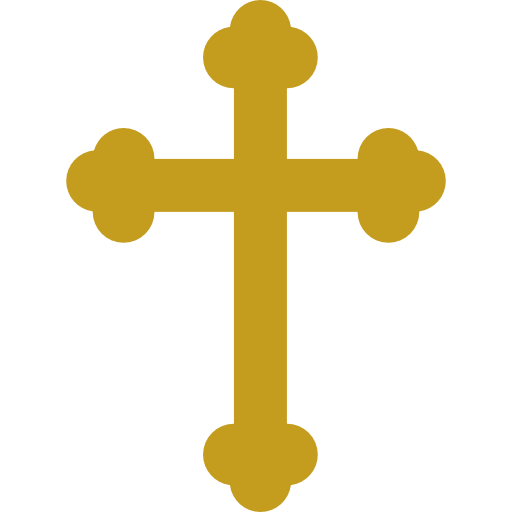
\includegraphics[scale=0.2]{assets/cross.png}\quad
  \textit{Novena a \textbf{Nossa Senhora de Nazaré}}
}
\fancyfoot[RO,RE]{\thepage}

\begin{document}


\subsection*{Novena a Nossa Senhora de Nazaré}

\say{
Conheço as festividades do Círio há mais de 18 anos. E posso afirmar com toda certeza: é a maior manifestação de fé e amor a Virgem Maria que já vi em toda a minha vida. Tive a graça de, por muitos anos seguidos, viver o Círio, esta é a palavra: “viver” o Círio de Nazaré. Pois não se participa, e sim vive-se. 
}


\begin{flushright}
--- Padre Bruno Costa 

Missionário da Comunidade Canção Nova.

\end{flushright}

\par\noindent\rule{\textwidth}{0.4pt}


\tableofcontents
\thispagestyle{empty}

% --- Vida / Origem da Novena ---
\newpage

\section{Origem da Devoção}

\subsection{Imagem de Nossa Senhora de Nazaré é escondida}

Com a invasão dos Mouros em Portugal, o rei Rodrigo, último rei visigodo da Península Ibérica, fugiu levando as relíquias de São Brás, São Bartolomeu e a imagem de Nossa Senhora de Nazaré, junto com sua família e com Frei Romano que sempre o acompanhou.

Antes de morrer, Frei Romano escondeu a imagem numa gruta. A imagem ficou ali por mais de 400 anos. Ela foi descoberta em 1182, por pastores que andavam pela região. Por causa da sua simplicidade, beleza e diferença dos padrões de imagens, Nossa Senhora de Nazaré voltou a ser venerada.

\subsection{Milagre de Nossa Senhora de Nazaré}

O cavaleiro Diego Fuas Roupinho, que era Alcaide do porto de Mós e Almirante de Dom Afonso, assim foi salvo por milagre de Nossa Senhora de Nazaré: Ele perseguia uma caça num dia de muita neblina. A caça caiu num abismo por causa da cerração. O cavaleiro não sabia que corria para o abismo. Mas, antes que caísse, ele vinha rezando a Senhora de Nazaré para que o protegesse.

De repente, então, o cavalo parou. A cerração se dissipou e ele viu que estava à beira de um abismo onde a caça tinha caído. Após esse milagre, a vila onde ocorreu passou a ser chamada de Vila de Nossa Senhora de Nazaré. Lá, foi construída uma pequena capela por Diego Roupinho, o cavaleiro salvo. Hoje existe ali uma grande Igreja em homenagem a Nossa Senhora.

\subsection{Devoção a Nossa Senhora de Nazaré }

Os Jesuítas foram os primeiros responsáveis em propagar a devoção de Nossa Senhora de Nazaré por toda a região de Portugal e posteriormente para toda a Europa. A principal casa de estudos e noviciado do mosteiro Jesuíta em Portugal é dedicada a Nossa Senhora de Nazaré.

\subsection{Devoção a Nossa Senhora de Nazaré no Brasil}

No dia 8 de setembro do ano de 1630, após uma grande tempestade, um pescador saiu para ver suas redes no mar de Saquarema. Ao passar diante de um morro, onde hoje está erguida a Igreja Matriz dedicada a Nossa Senhora de Nazaré, viu uma forte luz e foi verificar o que era. No local do brilho, ele encontrou a imagem de Nossa Senhora de Nazaré.

Levou a imagem para sua casa na vila dos pescadores, reuniu todos os pescadores, fizeram orações e foram dormir. No dia seguinte, a imagem reapareceu no local onde havia sido encontrada. Isso aconteceu por duas vezes.  Todos entenderam que era para construir uma capela naquele local. Muitos milagres aconteceram a partir de então e a capela ficou pequena, sendo necessário construir uma igreja bem maior. Sua festa é celebrada no dia 8 de setembro.

\subsection{O Círio de Nazaré em Belém do Pará}

Círio, cereus, é uma palavra que significa vela grande.  A devoção à Senhora de Nazaré foi levada para Belém do Pará pelos padres Jesuítas há mais de 200 anos e se tornou a maior festa católica do mundo dedicada à Mãe de Jesus.

A festa é celebrada desde 1793, e hoje, mais de 2 milhões de pessoas participam todos os anos.  É celebrada no segundo domingo de outubro.

Uma grande procissão com todos levando velas, sai de uma Igreja e faz o translado da imagem de Nossa Senhora de Nazaré para outra igreja, em um percurso de 5 quilômetros.

Existe também a procissão de carros, motos e a grande procissão de barcos.

\newpage

% --- Orações Diárias ---
\newpage

\section{Novena a Nossa Senhora de Nazaré}
\subsection{Oração Inicial} \label{sec:oracao-inicial}

Senhor, nosso Pai, estamos unidos em nome de Jesus, vosso Filho, conduzidos pelo Espírito Santo de Amor. Nós vos agradecemos pelo dom da fé cristã que nos reúne e pela Igreja que nos conduz pelos caminhos da vida felizes, nesta Terra e para a eternidade.

Pai eterno, Vós nos destes de presente a Virgem de Nazaré, Mãe de Jesus Cristo, Mãe da Igreja e nossa Mãe. Unidos a Maria, pedimos com confiança: envolve-nos com laços de amizade e com cordas de amor, trazei-nos para perto de vós, de Jesus Cristo e do Espírito Santo.

Acendei, ó Pai, em nossos corações, o Círio da Fé, da Esperança e da Caridade. Enchei nossos corações com a alegria do Evangelho. Que o povo de Nossa Senhora de Nazaré, Rainha e Padroeira da Amazônia, seja testemunha fiel do Evangelho Vivente – Jesus Cristo, para o crescimento de vosso Reino de paz e justiça, Reino de vida e verdade, Reino do amor e da graça. Amém.

\subsection{Primeiro Dia}

\textbf{\nameref{sec:oracao-inicial}}

Nossa Senhora de Nazaré, cuidai de nossas vidas.

“Todos os dons, virtudes e graças do Espírito Santo são distribuídos pelas mãos de Maria, a quem ela quer, quando quer, como quer, e quanto quer”. (São Bernardino de Sena)

Recolhamo-nos em oração nas nossas casas, com nossas famílias, com os que amamos e que estão longe fisicamente, ou rezemos sozinhos com o coração ardente pelo Amor à Maria.

\textbf{Em nome do Pai, do Filho e do Espírito Santo. Amém.}

Nossa Senhora de Nazaré, cuidai de nossas vidas:

Na cruz, Jesus, num gesto de grande doação, deu-nos Maria como mãe, mãe de toda a humanidade. “Tendo amado os seus que estavam no mundo, amou-os até o fim”. Quando Maria e o discípulo estão aos pés da cruz e o Senhor diz: “Eis aí tua mãe”, Ele foi se desprendendo de tudo. Não lhe restava mais que a sua mãe, e também a entrega à humanidade em sinal do seu amor por nós. Maria aos pés da cruz se apresenta cheia da serenidade do Filho, já participante da sua vitória. Cristo venceu morrendo. Maria, sofrendo. Que Maria nos acolha como filhos bem amados, e que cuide de nossas vidas, nos ensinando a fazer tudo o que Jesus disser.

\textbf{\nameref{sec:oracao-final}}

\subsection{Segundo Dia}

\textbf{\nameref{sec:oracao-inicial}}

Nossa Senhora cuida de nossa saúde.

“Tal é a vontade de Deus que quis que tenhamos tudo por Maria. Se portanto temos alguma esperança, alguma graça, algum dom salutar, saibamos que isto nos vem por suas mãos!” São Bernardo

Recolhamo-nos em oração nas nossas casas, com nossas famílias, com os que amamos e que estão longe fisicamente, ou rezemos sozinhos com o coração ardente pelo Amor à Maria.

\textbf{Em nome do Pai, do Filho e do Espírito Santo. Amém.}

Nossa Senhora de Nazaré, cuidai de nossa saúde

Mãe Santíssima ensina-nos a viver com plena saúde em todos os níveis: biológico, psíquico, social e espiritual; em contato permanente com o autor e fonte da vida que está na raiz do nosso ser; em harmonia com todos os seres humanos em sintonia com toda a criação. Interceda, Mãe querida, para que o teu Filho cure as nossas enfermidades, transforme as nossas lágrimas em oração e os nossos sofrimentos em momentos de crescimento, converta a nossa solidão em contemplação e a nossa espera em esperança, nos fortaleça na hora da agonia e transforme a nossa morte em ressurreição. Amém.

\textbf{\nameref{sec:oracao-final}}

\subsection{Terceiro Dia}

\textbf{\nameref{sec:oracao-inicial}}

Nossa Senhora de Nazaré, livrai-nos de todos os perigos

“Eu vos pertenço, Santíssima Virgem, salvai-me!” Salmo 118,94.

Recolhamo-nos em oração nas nossas casas, com nossas famílias, com os que amamos e que estão longe fisicamente, ou rezemos sozinhos com o coração ardente pelo Amor à Maria.

\textbf{Em nome do Pai, do Filho e do Espírito Santo. Amém.}

Nossa Senhora de Nazaré, livrai-nos de todos os perigos

O ícone de Maria que contemplamos enquanto oferece Jesus no Templo, prefigura o ícone da Crucifixão. Com efeito, é no Calvário que alcança o seu cumprimento, a oblação do Filho e, também a da Mãe. A mesma espada atravessa ambos, a Mãe e o Filho. A mesma dor, o mesmo amor. Ó Maria, Mãe de Cristo e nossa Mãe, agradecemos-te o cuidado com que nos acompanhas ao longo do caminho da vida, e te pedimos: “Neste momento difícil por qual passa toda a humanidade, ensina-nos a suportar a dor da alma transpassada, e intercede junto a Jesus para livrar-nos de todos os perigos, e se os tivermos que enfrentar, dê-nos força e coragem necessárias para suportar as provas da vida. Amém!

\textbf{\nameref{sec:oracao-final}}

\subsection{Quarto Dia}

\textbf{\nameref{sec:oracao-inicial}}

Nossa Senhora de Nazaré, curai os enfermos

Recolhamo-nos em oração nas nossas casas, com nossas famílias, com os que amamos e que estão longe fisicamente, ou rezemos sozinhos com o coração ardente pelo Amor à Maria.

\textbf{Em nome do Pai, do Filho e do Espírito Santo. Amém.}

Nossa Senhora de Nazaré, curai os enfermos

O chamado a evangelização e ao apostolado vem com uma responsabilidade, curar os doentes. Que Nossa Senhora de Nazaré nos ajude nesta missão que fomos enviados para curar os enfermos seja com nossos conhecimentos práticos (tal qual o evangelista São Lucas que era médico), seja com a oração ou com a evangelização. No tempo em que vivemos, que possamos estender a mão para os que mais necessitam e para os que estão próximos de nós precisando de amparo. Que a Virgem santíssima interceda por nós para que consigamos sempre ofertar ao irmão uma palavra de conforto e um sorriso amigo, dizendo-lhes: “O Reino de Deus está próximo de vós”. Amém.

\textbf{\nameref{sec:oracao-final}}

\subsection{Quinto Dia}

\textbf{\nameref{sec:oracao-inicial}}

Nossa Senhora de Nazaré, somos milagres, estamos aqui

“Aquela que era cheia de graça deixou transbordar essa graça sobre nós!” São Bernardo de Claraval

Recolhamo-nos em oração nas nossas casas, com nossas famílias, com os que amamos e que estão longe fisicamente, ou rezemos sozinhos com o coração ardente pelo Amor à Maria.

\textbf{Em nome do Pai, do Filho e do Espírito Santo. Amém.}

Nossa Senhora de Nazaré, somos milagres, estamos aqui

Mãe da Igreja, assim como pedistes ao teu Filho amado o milagre das Bodas de Caná, faça com que nós sejamos milagres e a serviço do Senhor. Que o Senhor opere seus milagres por meio de nós ao respondermos o chamado de Maria, fazendo tudo o que Ele nos disser. Que pensemos sobre nosso papel enquanto católicos para estarmos sempre a disposição de Deus, por meio da oração, nos prostrando diante Dele para que assim seja feita a sua vontade, e nossas obras cotidianas como água, se tornem milagres como vinho, por Cristo e com Maria. Amém.

\textbf{\nameref{sec:oracao-final}}

\subsection{Sexto Dia}

\textbf{\nameref{sec:oracao-inicial}}

Nossa Senhora de Nazaré, santificai-nos

“Todos somos chamados à santidade, e só os santos podem renovar a humanidade!” São João Paulo II

Recolhamo-nos em oração nas nossas casas, com nossas famílias, com os que amamos e que estão longe fisicamente, ou rezemos sozinhos com o coração ardente pelo Amor à Maria.

\textbf{Em nome do Pai, do Filho e do Espírito Santo. Amém.}

Nossa Senhora de Nazaré, santificai-nos:

Deus nos pede para sermos santos como Ele é. Para isso, temos que seguir o exemplo de Cristo, não nos prender aos bens perecíveis desse mundo, e sim ter fé na verdade Dele, o qual se encarnou e morreu na Cruz para nos salvar de nossos pecados. A partir desse ato supremo de amor de Deus por nós; Deus nos ensina a seguir o mandamento que Ele nos deixou, o qual foi o “amar a Deus sobre todas as coisas”, que só será pleno quando se ama o próximo, pois só ama verdadeiramente a Deus quem ama o próximo. Com essa atitude de amor possamos aprender que devemos buscar mudanças nas nossas atitudes e no nosso interior, para que nos tornemos santos. Façamos como Santa Teresinha do Menino Jesus que nos ensina, que mesmo distantes uns dos outros, podemos estar unidos, pois o que nos une é a ORAÇÃO. Portanto, pensar em uma pessoa que se ama é rezar por ela. Amém.

\textbf{\nameref{sec:oracao-final}}

\subsection{Setimo Dia}

\textbf{\nameref{sec:oracao-inicial}}

Nossa Senhora de Nazaré, dai-nos a graça.

“Deus juntou todas as águas e fez o mar. Reuniu todas as graças e as chamou de Maria!” São Luís Maria Grignion de Montfort

Recolhamo-nos em oração nas nossas casas, com nossas famílias, com os que amamos e que estão longe fisicamente, ou rezemos sozinhos com o coração ardente pelo Amor à Maria.

\textbf{Em nome do Pai, do Filho e do Espírito Santo. Amém.}

Nossa Senhora de Nazaré, dai-nos a graça

A Virgem Santíssima recebeu a graça de Deus de conceber seu Filho, e ela deu seu “Sim” com prontidão, o que nos deixa um exemplo de obediência a Deus. Há uma grandeza no “faça-se” dito por Maria, já que nesta palavra é onde melhor se faz transparente o modelo do cristão: o que se abre para dizer sim a Deus. Maria é remédio para a solidão e a desagregação. É a Mãe da consolação, por isso Ela sabe que, para consolar, não bastam as palavras; é necessária a presença. E Maria está presente como mãe. Permitamos-lhe que abrace a nossa vida. Nossa Mãe nos ajude a enfrentar com mais fé e esperança o tempo de provação que estamos atravessando. Que em tempos difíceis, nunca percamos a fé, e rezemos a Deus para que dias melhores possam vir. Que Nossa Senhora de Nazaré interceda por nós, passe na frente, nos dando a graça, protegendo a nossa vida, dos nossos familiares, dos profissionais de saúde, dos nossos sacerdotes de todo povo de Belém, do Brasil, e do mundo inteiro. Amém

\textbf{\nameref{sec:oracao-final}}

\subsection{Oitavo Dia}

\textbf{\nameref{sec:oracao-inicial}}

Nossa Senhora de Nazaré, ensinai-nos a servir.

“Esta grande compaixão de Maria para com nossas misérias a leva a nos socorrer e consolar, mesmo quando não a invocamos!” Santo Afonso de Ligório.

Recolhamo-nos em oração nas nossas casas, com nossas famílias, com os que amamos e que estão longe fisicamente, ou rezemos sozinhos com o coração ardente pelo Amor à Maria.

\textbf{Em nome do Pai, do Filho e do Espírito Santo. Amém.}

Nossa Senhora de Nazaré, ensinai-nos a servir

Mãe Santíssima, que, inspirados em vossa visita à prima Isabel logo após o anúncio da encarnação de Cristo, possamos despir-nos da preocupação com o nosso próprio conforto e pormo-nos, com prontidão, a serviço dos nossos irmãos, em atitude de desprendimento, zelo e cuidado, fazendo-nos também seus intercessores e auxiliadores. Que, tal como o fizestes com a família de Isabel, ofereçamos o próprio Cristo aos nossos irmãos, por meio do serviço solidário. Que, a vosso exemplo Ó Boa Mãe, sejamos instrumentos do infinito amor de Deus, levando paz e esperança aos nossos irmãos aflitos.

\textbf{\nameref{sec:oracao-final}}

\subsection{Nono Dia}

\textbf{\nameref{sec:oracao-inicial}}

Nossa Senhora de Nazaré, transformai-nos em cristãos mais atentos ao próximo.

“A quem Deus quer fazer muito santo, o faz muito devoto da Virgem Maria!” São Luís Maria Grignion de Montfort

Recolhamo-nos em oração nas nossas casas, com nossas famílias, com os que amamos e que estão longe fisicamente, ou rezemos sozinhos com o coração ardente pelo Amor à Maria.

\textbf{Em nome do Pai, do Filho e do Espírito Santo. Amém.}

Nossa Senhora de Nazaré, transformai-nos em cristãos mais atentos ao próximo

Mãe Santíssima, com a Graça do Altíssimo, faça-nos viver plenamente a Lei da Caridade. Livre-nos da indiferença e do medo, da frieza e do descaso perante as misérias da vida. Faze-nos corajosos e ativos para carregar a nossa Cruz diária. Não nos deixe fugir da dor, ao contrário, faze-nos aceitá-la para que sejamos por ela curados. Prepara-nos para todas as tribulações, para que com elas possamos amadurecer e completar na carne os sofrimentos do teu filho Jesus. Fazei brotar em nossos corações a mesma chama que brotou no coração do bom samaritano, para que possamos verdadeiramente amar a Deus em nossos irmãos feridos. Amém.

\textbf{\nameref{sec:oracao-final}}

\newpage

\subsection{Oração Final} \label{sec:oracao-final}

Ó Virgem Imaculada de Nazaré, fostes na terra criatura tão humilde, a ponto de dizer ao Anjo Gabriel: Eis aqui a escrava do Senhor. Mas, por Deus fostes exaltada, e preferida entre todas as mulheres, para exercer a sublime missão de Mãe do Verbo Encarnado. Adoro e louvo ao Altíssimo que vos elevou a essa excelsa dignidade e vos preservou da culpa original.

Quanto a mim, soberbo e carregado de pecados, sinto-me confundido e envergonhado perante vós. Entretanto, confiando na bondade e ternura de vosso Coração Imaculado e maternal, peço-vos a força de imitar a vossa humildade, e participar da vossa caridade a fim de viver unido, pela graça, ao vosso divino filho Jesus. Assim como vós viveste no retiro de Nazaré.

Para alcançar essa graça, \textbf{(fazer o pedido com fé...)}, quero com imenso afeto, e filial devoção, saudar-vos como o Arcanjo Gabriel: \textbf{Ave-Maria}...

\response Rogai por nós, Santa Mãe de Deus,

\versicle Para que possamos aprofundar nossa dedicação ao vosso Filho e reavivar o mundo com o seu Espírito. 


\vfill

\begin{center}
\subsection*{Fontes:}
Adaptado de: 
\begin{itemize}
  \item \underline{\href{https://cruzterrasanta.com.br/historia-de-nossa-senhora-nazare/48/102}{Cruz Terra Santa}}\\
    \item \underline{\href{https://www.miliciadaimaculada.org.br/espiritualidade/santos/novena-nossa-senhora-nazare}{Milícia da Imaculada - Novena a Nossa Senhora de Nazaré}}\\
    \item \underline{\href{https://santuario.cancaonova.com/artigos-religiosos/padre-relata-sua-experiencia-com-o-cirio-de-nazare/}{Canção Nova}}\\

\end{itemize}
\end{center}


\end{document}
